\documentclass[11pt,a4paper]{article}
\usepackage[spanish,es-tabla]{babel}
\usepackage[utf8]{inputenc}
\usepackage[T1]{fontenc}
\usepackage{lmodern}
\usepackage[margin=2.3cm]{geometry}
\usepackage{graphicx,booktabs,float,caption,subcaption,xcolor,listings,tabularx,enumitem,amsmath,array,multirow}
\usepackage{tikz,pgfplots}
\usetikzlibrary{automata,positioning,arrows.meta}
\pgfplotsset{compat=1.18}
\usepackage[hidelinks]{hyperref}
\usepackage{fancyhdr}

\definecolor{nuevo}{RGB}{220,110,10}
\definecolor{codebg}{RGB}{246,246,246}
\lstdefinelanguage{Verilog}{
  morekeywords={module,endmodule,input,output,wire,reg,assign,always,begin,end,if,else,posedge,negedge,or,parameter,localparam,integer,for,case,endcase},
  sensitive=true, morecomment=[l]{//}, morestring=[b]"}
\lstset{language=Verilog, basicstyle=\ttfamily\footnotesize, keywordstyle=\color{blue!60!black}\bfseries,
  backgroundcolor=\color{codebg}, frame=single, rulecolor=\color{gray!40}, columns=fullflexible,
  keepspaces=true, showstringspaces=false, breaklines=true, xleftmargin=4pt, xrightmargin=4pt,
  literate={á}{{\'a}}1 {é}{{\'e}}1 {í}{{\'i}}1 {ó}{{\'o}}1 {ú}{{\'u}}1 {ñ}{{\~n}}1}

\pagestyle{fancy}
\fancyhf{}
\fancyhead[L]{\small Arquitectura de Computadoras — Proyecto 2}
\fancyhead[R]{\small Entrega final}
\fancyfoot[C]{\thepage}
\renewcommand{\headrulewidth}{0.4pt}

\captionsetup{font=small,labelfont=bf}
\setlength{\parskip}{4pt}

\newcommand{\sig}[1]{\texttt{#1}}

\begin{document}

\begin{titlepage}
\centering
\vspace*{1.2cm}
{\Large Arquitectura de Computadoras\par}
\vspace{3cm}
{\huge\bfseries Diseño e implementación de un procesador\\[4pt] RISC-V superescalar Dual-Issue con\\[4pt] optimización microarquitectónica\par}
\vspace{2cm}
{\Large Proyecto 2 – Entrega final\par}
\vspace{0.6cm}
{\large Optimización: Branch Target Buffer con predictor de 2 bits\par}
\vspace{3cm}
{\large\bfseries Integrantes\par}
\vspace{0.4cm}
\begin{tabular}{ll}
Alvarez Lovera, Sandra Sofia & 202510738 \\
Gutierrez Rodriguez, Mahir Gianpier & 202510475 \\
Alva Espinoza, Jose Luis & 202420038 \\
\end{tabular}
\vfill
{\large 2026 – 2\par}
\end{titlepage}

\tableofcontents
\newpage

\section*{Resumen}
\addcontentsline{toc}{section}{Resumen}

Esta entrega completa el proyecto con la versión optimizada del procesador Dual-Issue in-order construido en E1 y E2. La limitación elegida es el costo de los saltos tomados: en el Dual-Issue se resuelven en Execute y cada uno anula las etapas F y D, es decir, hasta cuatro slots de emisión. La optimización implementada es un \textbf{Branch Target Buffer (BTB) de 16 entradas con un contador saturado de 2 bits por entrada}, consultado en Fetch para las dos instrucciones del paquete. Con la predicción, el procesador solo vacía el pipeline cuando la predicción falla.

Las tres arquitecturas —(A) pipeline Single-Issue, (B) Dual-Issue y (C) Dual-Issue optimizado— ejecutan sin modificaciones el programa del profesor y un programa propio, y en los dos casos producen exactamente el mismo estado arquitectónico. La Tabla~\ref{tab:resumen} resume el resultado principal.

\begin{table}[H]
\centering
\begin{tabular}{lrrrrrr}
\toprule
 & \multicolumn{3}{c}{Programa del profesor} & \multicolumn{3}{c}{Programa propio} \\
\cmidrule(lr){2-4}\cmidrule(lr){5-7}
 & A & B & C & A & B & C \\
\midrule
Ciclos & 458 & 387 & \textbf{292} & 583 & 437 & \textbf{373} \\
IPC & 0.681 & 0.806 & \textbf{1.068} & 0.840 & 1.121 & \textbf{1.314} \\
Speedup vs.\ A & 1.00 & 1.18 & \textbf{1.57} & 1.00 & 1.33 & \textbf{1.56} \\
Speedup vs.\ B & — & 1.00 & \textbf{1.33} & — & 1.00 & \textbf{1.17} \\
\bottomrule
\end{tabular}
\caption{Resultado principal de las tres arquitecturas.}
\label{tab:resumen}
\end{table}

\section{Punto de partida: las tres arquitecturas}

\subsection{(A) Pipeline Single-Issue y (B) Dual-Issue}

La arquitectura A es el pipeline RV32I de cinco etapas de la E1, con forwarding desde M y W, stall por load-use y flush ante saltos tomados. La arquitectura B es el procesador Dual-Issue in-order de la E2, cuyas características principales son:
\begin{itemize}[nosep]
  \item Dual Fetch (PC y PC+4) y dual decode, con dos \sig{controller}.
  \item Una \textbf{Issue Unit} que emite el par completo salvo que exista RAW dentro del par (\sig{RAWpar}), dos accesos a memoria (\sig{DosMem}) o dos saltos (\sig{DosSaltos}). Si solo sale la instrucción más antigua, la más joven se \emph{reagrupa}: pasa a la vía 1 y entra la siguiente instrucción como vía 2, sin pérdidas ni duplicados.
  \item Dos ALU, un Register File de 4 lecturas y 2 escrituras (la vía 2 escribe después de la vía 1), un único puerto de memoria de datos (\sig{MemSelM}) y una única unidad de saltos (\sig{BrSelE}).
  \item Una Hazard Unit con forwarding desde cuatro productores con prioridad M2~$>$~M1~$>$~W2~$>$~W1, stall por load-use en cualquiera de las vías y \sig{FlushM2} para anular la vía 2 cuando el salto tomado está en la vía 1.
\end{itemize}

\subsection{Cambios comunes para la entrega final}

El programa del profesor tiene 90 instrucciones y usa \sig{x1~=~1536} como base de datos, lo que no cabía en las memorias de 64 palabras de las entregas anteriores. En las tres versiones, por igual, se amplió la \sig{imem} a 256 palabras (índice \sig{a[9:2]}) y la \sig{dmem} a 512 palabras (índice \sig{a[10:2]}). Así, la dirección 1536 corresponde a \sig{RAM[384]} y no depende de un \emph{aliasing}. Con este cambio, todos los testbenches de E2 siguen pasando.

\section{Optimización: BTB con predictor de 2 bits}

\subsection{Limitación identificada}

En B, el salto se resuelve en Execute. Cuando es tomado, las instrucciones que ya entraron a F y D son del camino incorrecto y se anulan. En un pipeline escalar se pierden dos ciclos. En el Dual-Issue se pierden \emph{dos ciclos de dos slots cada uno}: hasta cuatro instrucciones que podrían haberse emitido.

El programa del profesor muestra el tamaño del problema: de 312 instrucciones retiradas, 89 son de control y 67 se toman. La etapa C, formada casi solo por lazos, ocupa 287 de los 387 ciclos de B. En esa etapa el Dual-Issue apenas mejora al pipeline (287 frente a 330 ciclos), porque el beneficio de emitir dos instrucciones se pierde en los flushes.

\subsection{Fundamento}

La idea es \textbf{predecir en Fetch} el siguiente PC en vez de esperar a Execute:
\begin{itemize}[nosep]
  \item El \textbf{BTB} guarda, para cada salto ya visto, su dirección destino. Al consultarlo con el PC se sabe si la instrucción es un salto y a dónde va, antes de decodificarla.
  \item El \textbf{contador saturado de 2 bits} decide si se predice tomado (estados 10 y 11) o no tomado (00 y 01). Hacen falta dos fallos seguidos para cambiar la predicción, lo que tolera la única salida de un lazo (Figura~\ref{fig:fsm}).
\end{itemize}

Si la predicción acierta, el salto no cuesta ningún ciclo. Si falla, el costo es el mismo que en B. La verificación se hace en Execute, donde ya se calculaban \sig{PCSrcE} y \sig{PCTargetE}.

\begin{figure}[H]
\centering
\begin{tikzpicture}[->,>={Stealth[length=2.2mm]}, node distance=2.6cm, every state/.style={minimum size=13mm, font=\small, thick}, font=\small]
  \node[state, fill=red!10] (s0) {00};
  \node[state, fill=red!5, right of=s0] (s1) {01};
  \node[state, fill=green!5, right of=s1] (s2) {10};
  \node[state, fill=green!10, right of=s2] (s3) {11};
  \path (s0) edge[bend left] node[above]{T} (s1)
        (s1) edge[bend left] node[above]{T} (s2)
        (s2) edge[bend left] node[above]{T} (s3)
        (s3) edge[loop right] node{T} (s3)
        (s3) edge[bend left] node[below]{NT} (s2)
        (s2) edge[bend left] node[below]{NT} (s1)
        (s1) edge[bend left] node[below]{NT} (s0)
        (s0) edge[loop left] node{NT} (s0);
  \node[below=0.9cm of s0, xshift=1.3cm, font=\footnotesize] {predice \textbf{no tomado}};
  \node[below=0.9cm of s2, xshift=1.3cm, font=\footnotesize] {predice \textbf{tomado}};
\end{tikzpicture}
\caption{Contador saturado de 2 bits. Una entrada nueva empieza en 10 si es un \sig{beq} y en 11 si es un \sig{jal}.}
\label{fig:fsm}
\end{figure}

\subsection{Diseño e implementación}

La Figura~\ref{fig:datapath} muestra el datapath de C. Los bloques en naranja son los que se agregan respecto de B.

\begin{figure}[H]
\centering
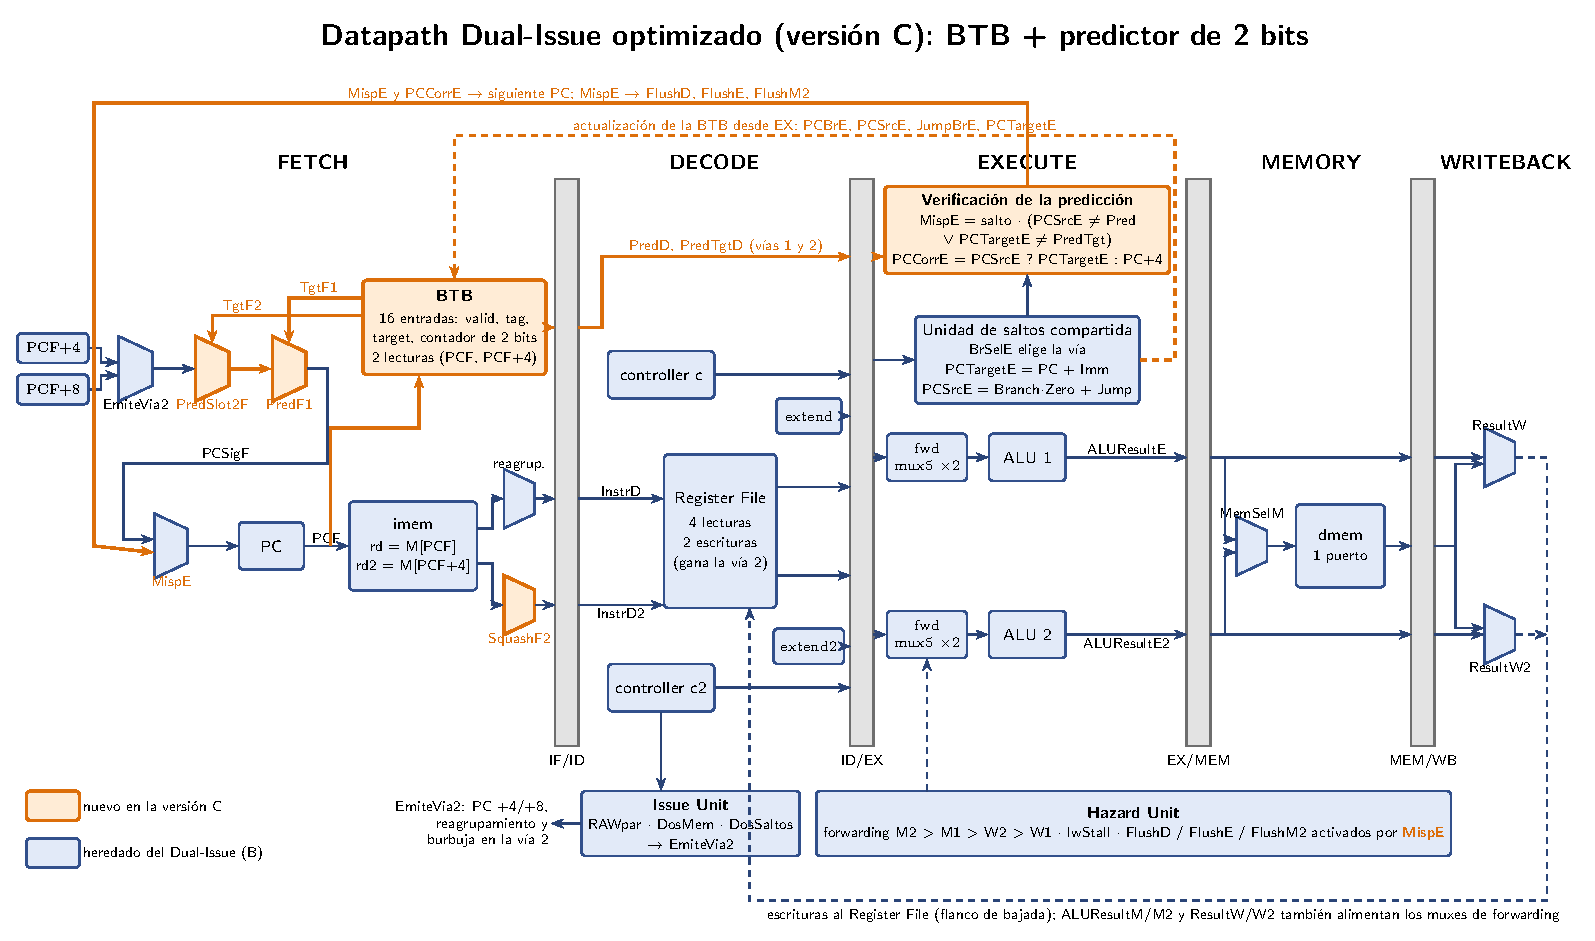
\includegraphics[angle=90,height=0.86\textheight]{datapath_C.pdf}
\caption{Datapath Dual-Issue optimizado. En naranja: BTB, muxes de predicción en Fetch, \sig{SquashF2}, registros de predicción (\sig{predregD/D2/E/E2}), verificación en Execute (\sig{MispE}, \sig{PCCorrE}) y actualización del BTB.}
\label{fig:datapath}
\end{figure}

\subsubsection{Módulos modificados}

\begin{table}[H]
\centering
\small
\begin{tabularx}{\textwidth}{>{\ttfamily}l X}
\toprule
\normalfont\textbf{Archivo} & \textbf{Cambio} \\
\midrule
btb.v & Módulo nuevo. 16 entradas de mapeo directo con índice \sig{PC[5:2]} y tag \sig{PC[31:6]}; cada entrada guarda valid, tag, target y contador. Dos puertos de lectura combinacionales (slots 1 y 2 del paquete) y uno de actualización síncrono desde Execute. \\
flopenrc.v & Módulo nuevo: registro con enable y clear, usado para llevar \sig{\{Pred, PredTgt\}} por IF/ID e ID/EX en las dos vías. \\
datapath.v & Siguiente PC predicho en Fetch, anulación del slot 2 (\sig{SquashF2}), registros de predicción, verificación \sig{MispE} y PC de corrección \sig{PCCorrE} en Execute. El mux del PC pasa a usar \sig{MispE} en lugar de \sig{PCSrcE}. \\
hazard\_unit.v & \sig{FlushD}, \sig{FlushE}, \sig{FlushM2} y la condición de \sig{StallF}/\sig{StallD} dependen de \sig{MispE} en lugar de \sig{PCSrcE}. \\
riscvpipeline.v & Conexión de \sig{MispE} entre el datapath y la Hazard Unit. \\
\bottomrule
\end{tabularx}
\caption{Archivos modificados en la versión C. El resto es idéntico a B.}
\end{table}

\subsubsection{Siguiente PC en Fetch}

El BTB se consulta con \sig{PCF} (slot 1) y \sig{PCF+4} (slot 2). La decisión tiene en cuenta qué instrucciones del fetch entran realmente a Decode, lo que depende del reagrupamiento:
\begin{itemize}[nosep]
  \item Si \sig{EmiteVia2~=~1}, entran \sig{InstrF} e \sig{InstrF2}. Si el slot 1 predice tomado, el PC salta a \sig{TgtF1} y el slot 2, que es camino incorrecto, entra como burbuja (\sig{SquashF2}). Si solo el slot 2 predice tomado (\sig{PredSlot2F}), el PC salta a \sig{TgtF2}. En otro caso, PC+8.
  \item Si \sig{EmiteVia2~=~0}, solo entra \sig{InstrF}, como vía 2 reagrupada. Si predice tomado, el PC salta a \sig{TgtF1}; si no, PC+4.
\end{itemize}

\begin{lstlisting}
assign SquashF2   = EmiteVia2 & PredF1;
assign PredSlot2F = EmiteVia2 & ~PredF1 & PredF2;
// pcseqmux: EmiteVia2 ? PCF+8 : PCF+4  ->  pcpred2mux: TgtF2  ->  pcpredmux: TgtF1
\end{lstlisting}

El reagrupamiento no necesita casos especiales. Si un salto predicho tomado se queda en la vía 2 de Decode porque la Issue Unit no lo dejó salir, el fetch ya se redirigió a su destino en el ciclo anterior. Por eso la instrucción que se reagrupa con él siempre es la del camino predicho.

\subsubsection{Verificación en Execute y actualización del BTB}

La predicción viaja con cada instrucción (\sig{PredD}/\sig{PredE} y \sig{PredTgtD}/\sig{PredTgtE}). La unidad de saltos compartida elige la vía del salto con \sig{BrSelE}, igual que en B, y compara:

\begin{lstlisting}
assign EsSaltoE = BranchBrE | JumpBrE;
assign MispE    = EsSaltoE & ((PCSrcE != PredBrE) | (PCSrcE & (PCTargetE != PredTgtBrE)));
// PCCorrE = PCSrcE ? PCTargetE : PC+4 del salto
\end{lstlisting}

Si \sig{MispE~=~1}, el PC se corrige y se anulan las instrucciones más jóvenes: F y D con \sig{FlushD}/\sig{FlushE}, y además la vía 2 de Execute con \sig{FlushM2} si el salto está en la vía 1. Así se respeta la regla del enunciado: si el salto está en la vía 2, la instrucción de la vía 1 es más antigua y se conserva. En el mismo ciclo, el BTB se actualiza con el resultado real: si el salto no tenía entrada y fue tomado, se crea una (contador 10 para \sig{beq} y 11 para \sig{jal}); si ya existía, el contador sube o baja con saturación.

\subsubsection{Costo de hardware}

\begin{itemize}[nosep]
  \item BTB: $16 \times (1 + 26 + 32 + 2) = 976$ bits de almacenamiento.
  \item Registros de predicción: $4 \times 33 = 132$ flip-flops (IF/ID e ID/EX, dos vías).
  \item Lógica: dos comparadores de tag de 26 bits en Fetch, uno en Execute para la actualización, un comparador de 32 bits para el target y cuatro muxes de 32 bits (cadena del siguiente PC, corrección y anulación).
\end{itemize}

La consulta al BTB y la cadena de tres muxes se suman al camino crítico de Fetch. En este trabajo se compara con el mismo periodo de reloj para las tres versiones, como indica el enunciado. En una implementación real habría que confirmar que la frecuencia no baja.

\section{Metodología de verificación y medición}

\paragraph{Testbench con modelo de commit.} Los testbenches de los dos programas (\sig{tb\_prog\_profesor.v}, \sig{tb\_prog\_propio.v}) mantienen un banco de registros sombra que se actualiza con cada instrucción que llega válida a Writeback, en orden de programa (vía 1 y luego vía 2). Cuando se retira la última instrucción de cada etapa, el testbench compara los 31 registros y la región de memoria con el estado de referencia y genera un pulso \sig{chk\_X}; \sig{ok\_X~=~1} indica que todo coincide. Como el criterio no depende de la temporización, el mismo testbench sirve para A, B y C.

\paragraph{Criterio de medición.} Los ciclos se cuentan desde que baja \sig{reset} hasta que se retira la última instrucción útil, y se excluye el lazo \sig{fin}. Las instrucciones retiradas son las que llegan válidas (\sig{Instr~$\neq$~0}) a Writeback. Las tres versiones usan las mismas memorias, el mismo testbench y el mismo periodo de reloj.

\paragraph{Validación adicional.}
\begin{itemize}[nosep]
  \item Los testbenches de E2 pasan en las versiones correspondientes (los de Single-Issue en A y los de Dual-Issue en B) y también en C.
  \item Prueba diferencial aleatoria: 400 programas generados al azar (lazos anidados, saltos hacia adelante, \sig{jal}, load-use, conflictos de memoria). En los 400, el estado final de A, B y C coincide con el de un modelo ISA escrito en Python.
  \item Todas las simulaciones se reprodujeron en Vivado (\sig{xvlog}/\sig{xelab}/\sig{xsim} 2025.2) con resultados idénticos ciclo a ciclo.
\end{itemize}

\section{Programa del profesor}

\subsection{Estados finales de las etapas A–D}

Las tres arquitecturas alcanzan los cuatro estados de referencia del enunciado. La Tabla~\ref{tab:etapas} indica el ciclo en que se verifica cada etapa. En la etapa D, el estado final es: x19~=~6, x20~=~6, x25~=~4, x26~=~4, x27~=~1560, x28~=~74, x29~=~4, x30~=~23, x31~=~1, M[x1+36]~=~74, M[x1+40]~=~4, M[x1+44]~=~0, M[x1+48]~=~1 y M[x1+52]~=~1, además de los valores de las etapas anteriores.

\begin{table}[H]
\centering
\begin{tabular}{lcccc}
\toprule
Versión & Etapa A & Etapa B & Etapa C & Etapa D \\
\midrule
A — Pipeline & 17 & 31 & 361 & 458 \\
B — Dual-Issue & 11 & 25 & 312 & 387 \\
C — Optimizado & 11 & 25 & 220 & 292 \\
\midrule
Resultado & OK & OK & OK & OK \\
\bottomrule
\end{tabular}
\caption{Ciclo en que se verifica cada etapa. La diferencia entre B y C se concentra en la etapa C, que está formada por lazos.}
\label{tab:etapas}
\end{table}

\subsection{Waveforms de cierre de etapa (versión C)}

Cada figura muestra el instante de comprobación con el cursor sobre el pulso \sig{chk\_X}. La parte superior muestra \sig{ciclos}, \sig{retiradas}, \sig{chk/ok} y los registros; la inferior, los registros restantes y la memoria (\sig{M0}…\sig{M52}~=~\sig{M[x1+0]}…\sig{M[x1+52]}). Los valores relevantes se leen en la columna \emph{Value}.

\begin{figure}[H]
\centering
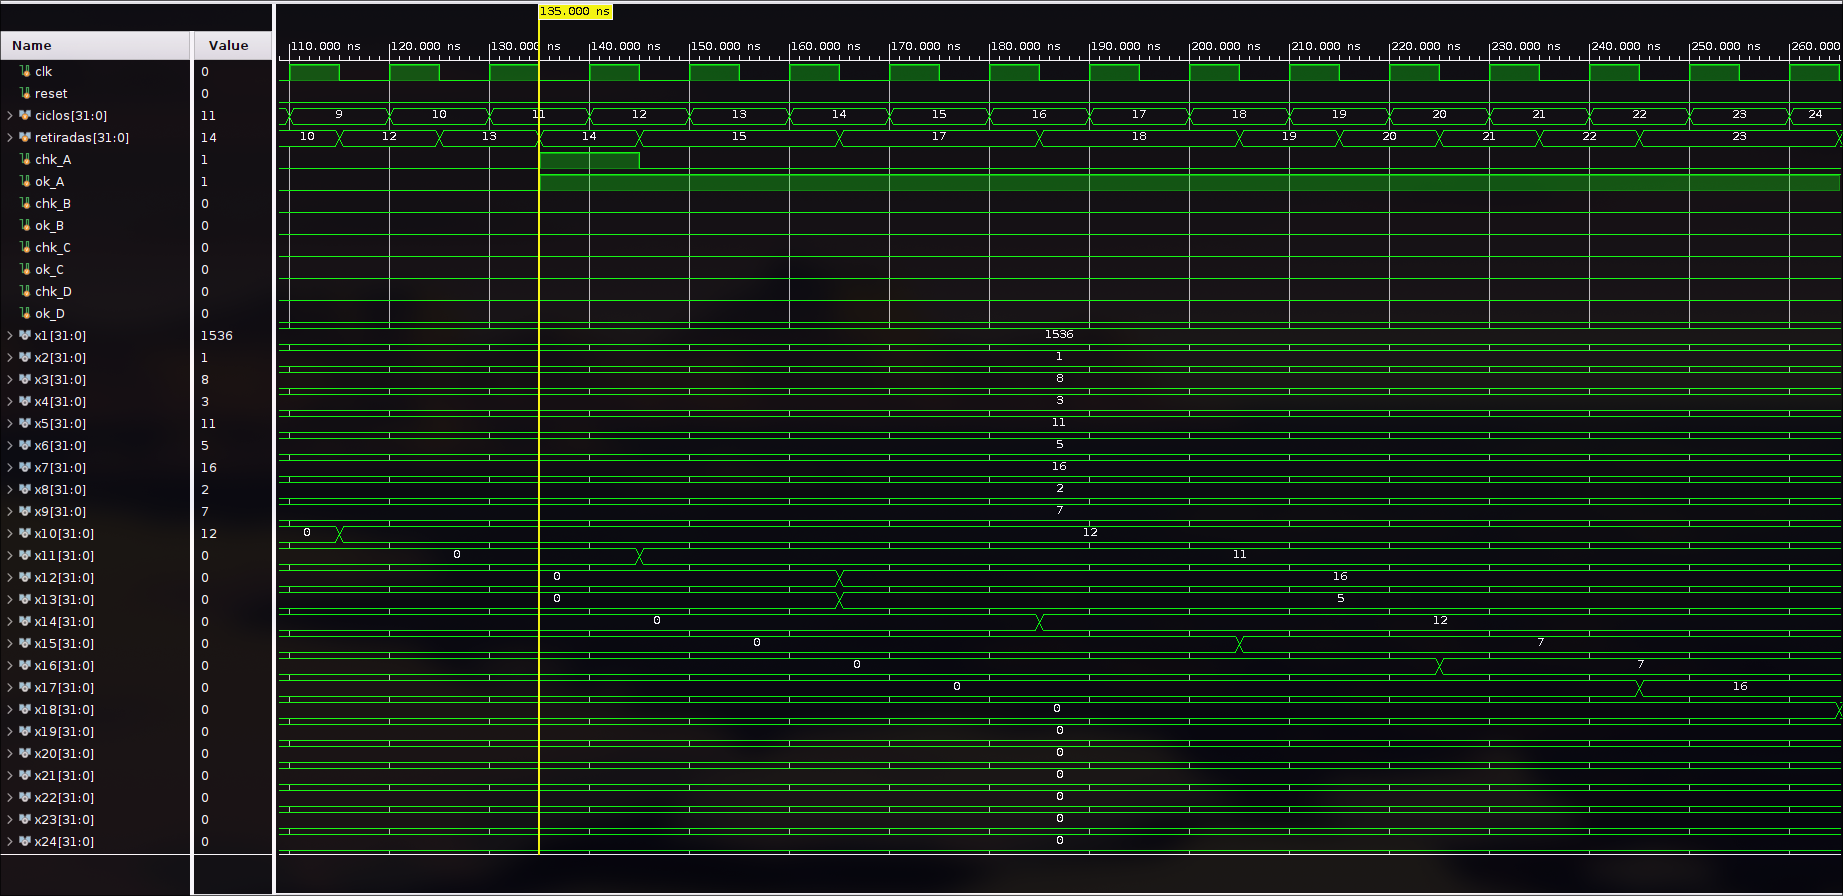
\includegraphics[width=\textwidth]{capturas/w1a_etapa_A.png}\\[2pt]
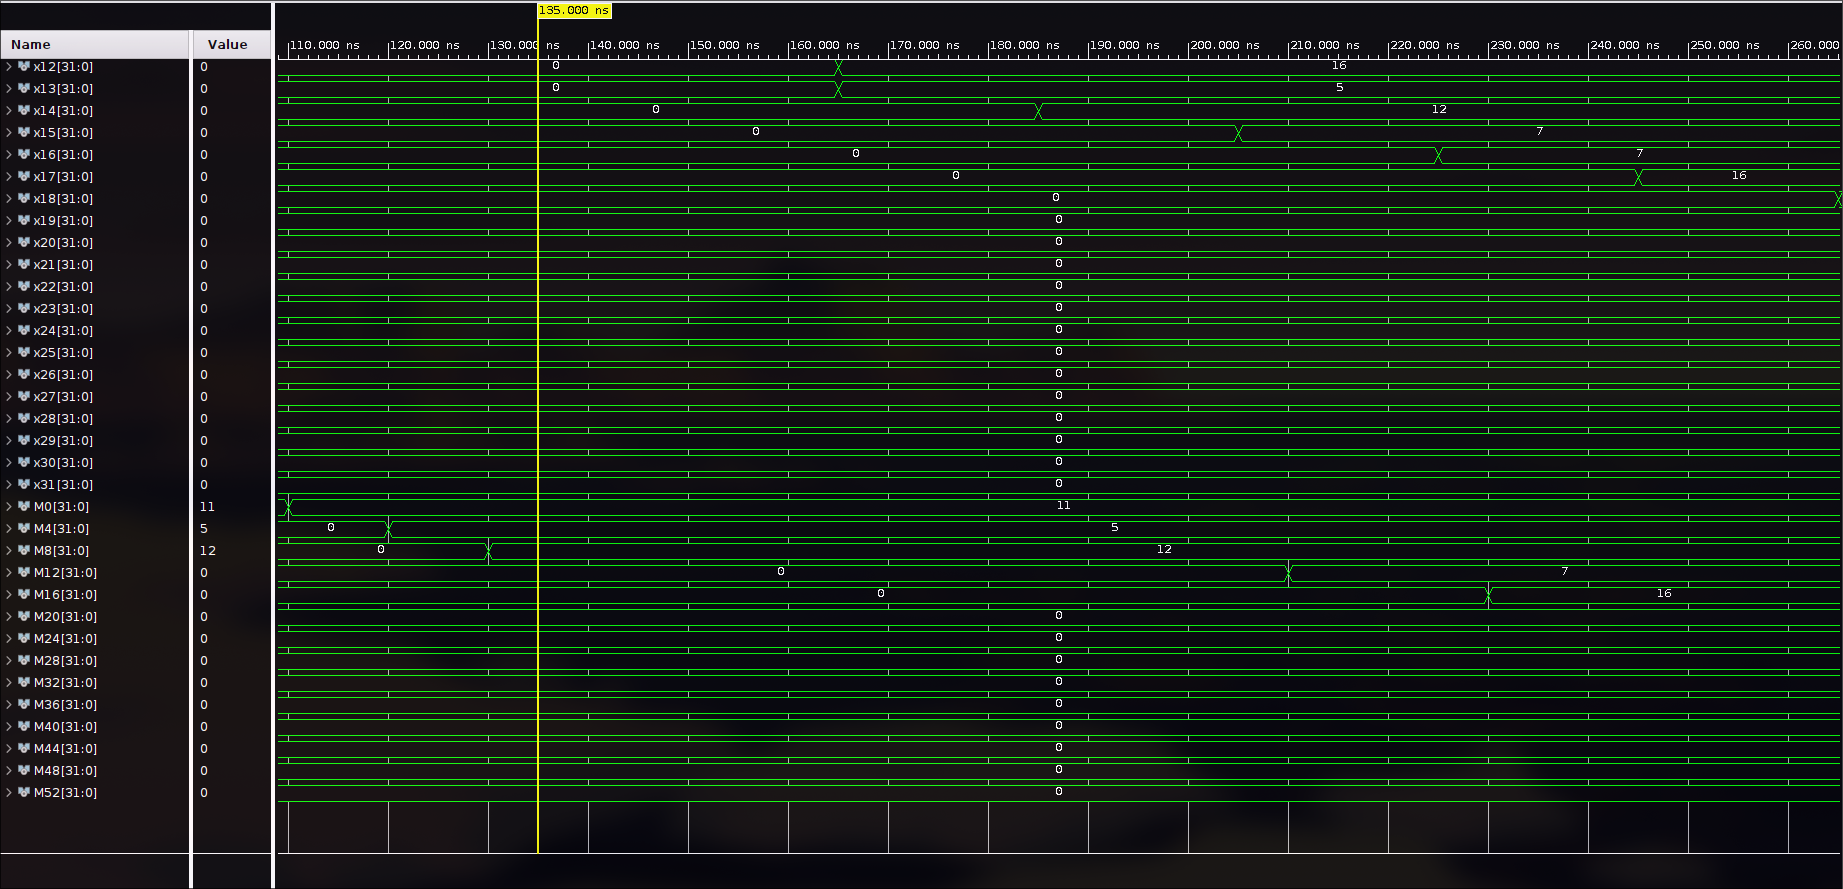
\includegraphics[width=\textwidth]{capturas/w1a_mem.png}
\caption{Cierre de la etapa A (135~ns, ciclo 11, 14 instrucciones retiradas). x5~=~11, x6~=~5, x7~=~16, x9~=~7 y x10~=~12; M0~=~11, M4~=~5 y M8~=~12; el resto de registros y memoria en 0. \sig{ok\_A~=~1}.}
\end{figure}

\begin{figure}[H]
\centering
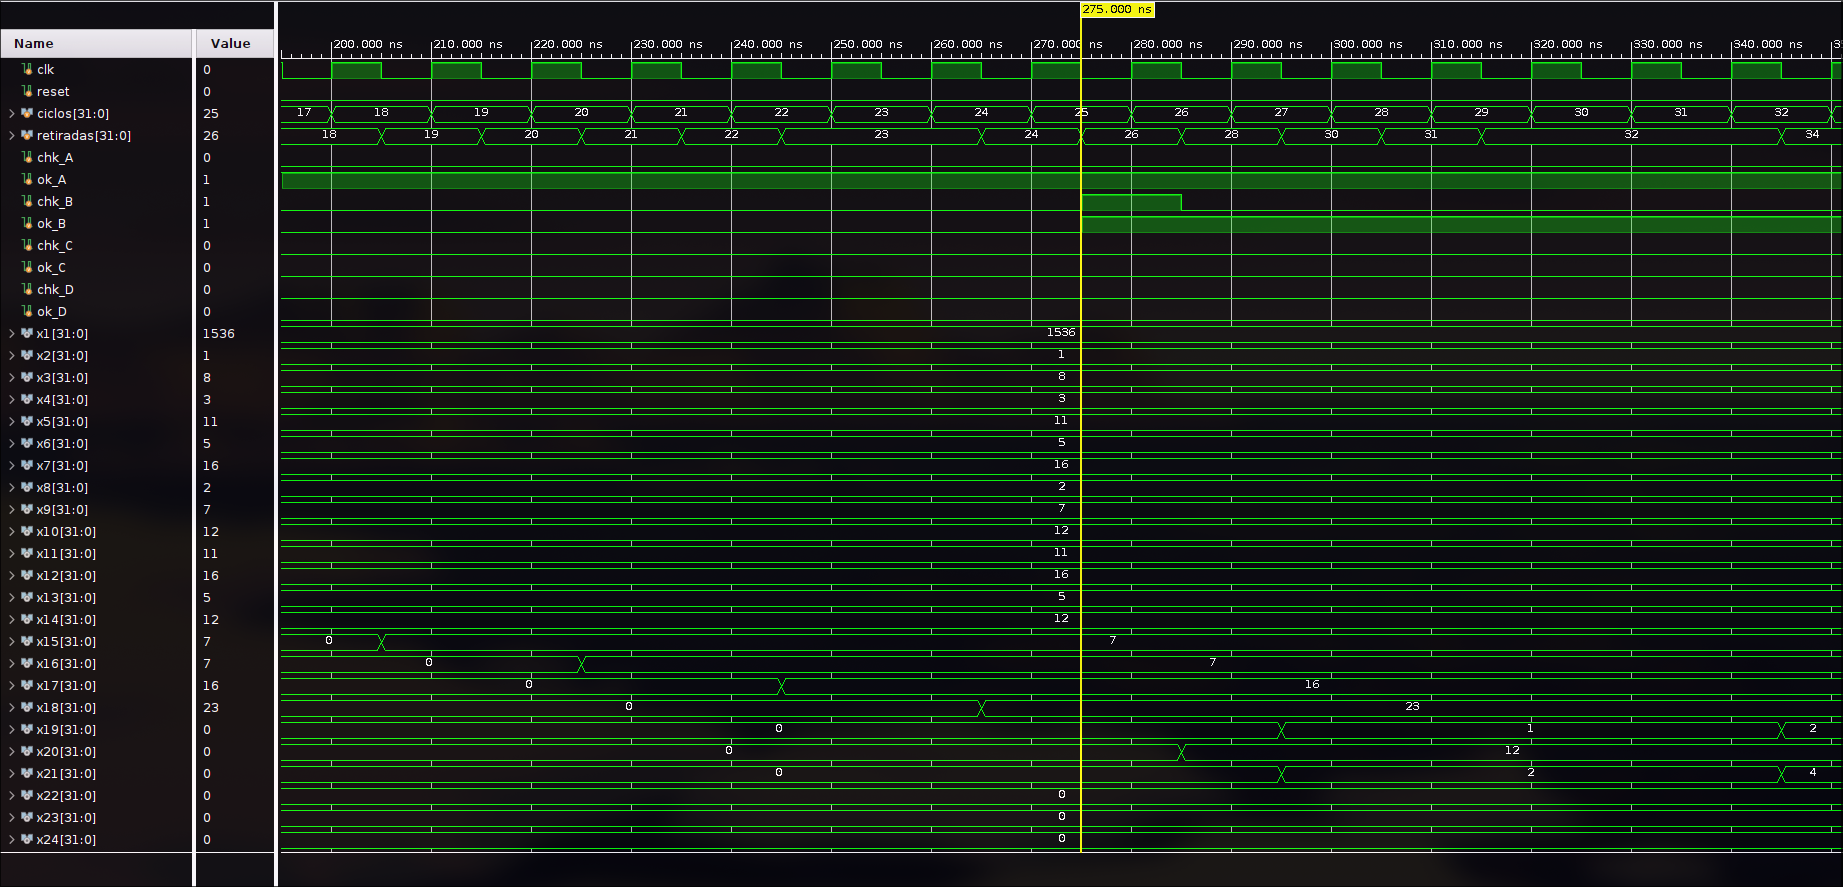
\includegraphics[width=\textwidth]{capturas/w1b_etapa_B.png}\\[2pt]
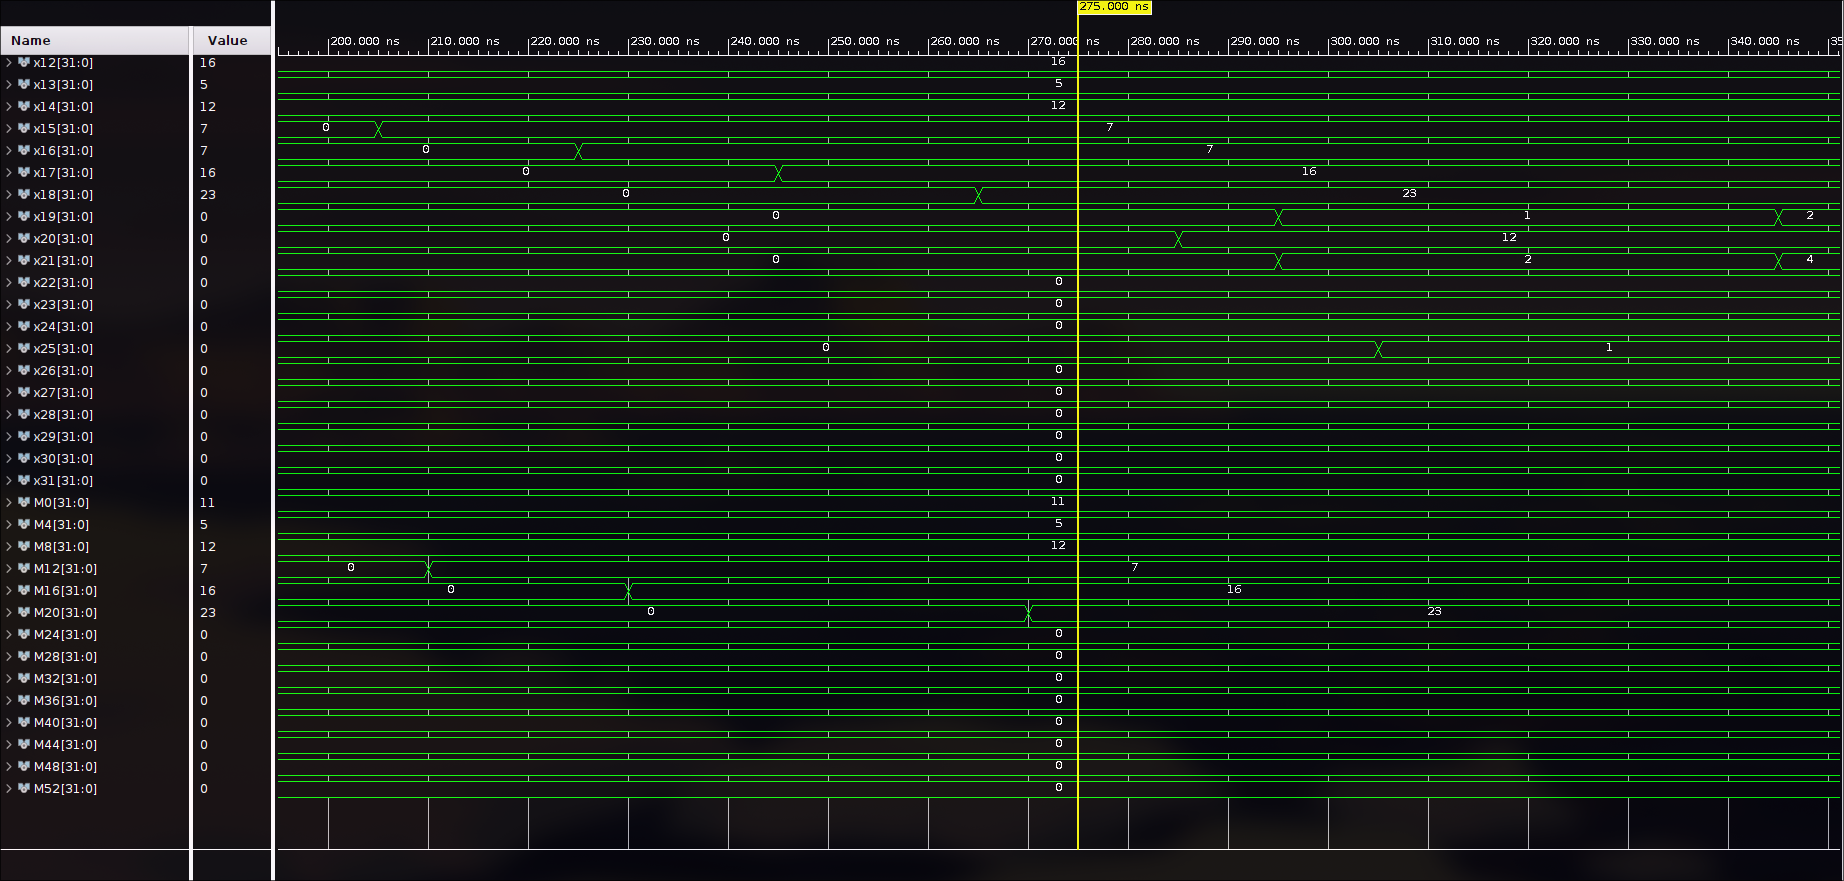
\includegraphics[width=\textwidth]{capturas/w1b_mem.png}
\caption{Cierre de la etapa B (275~ns, ciclo 25). x11~=~11, x12~=~16, x13~=~5, x14~=~12, x15~=~7, x16~=~7, x17~=~16 y x18~=~23; M12~=~7, M16~=~16 y M20~=~23. \sig{ok\_B~=~1}.}
\end{figure}

\begin{figure}[H]
\centering
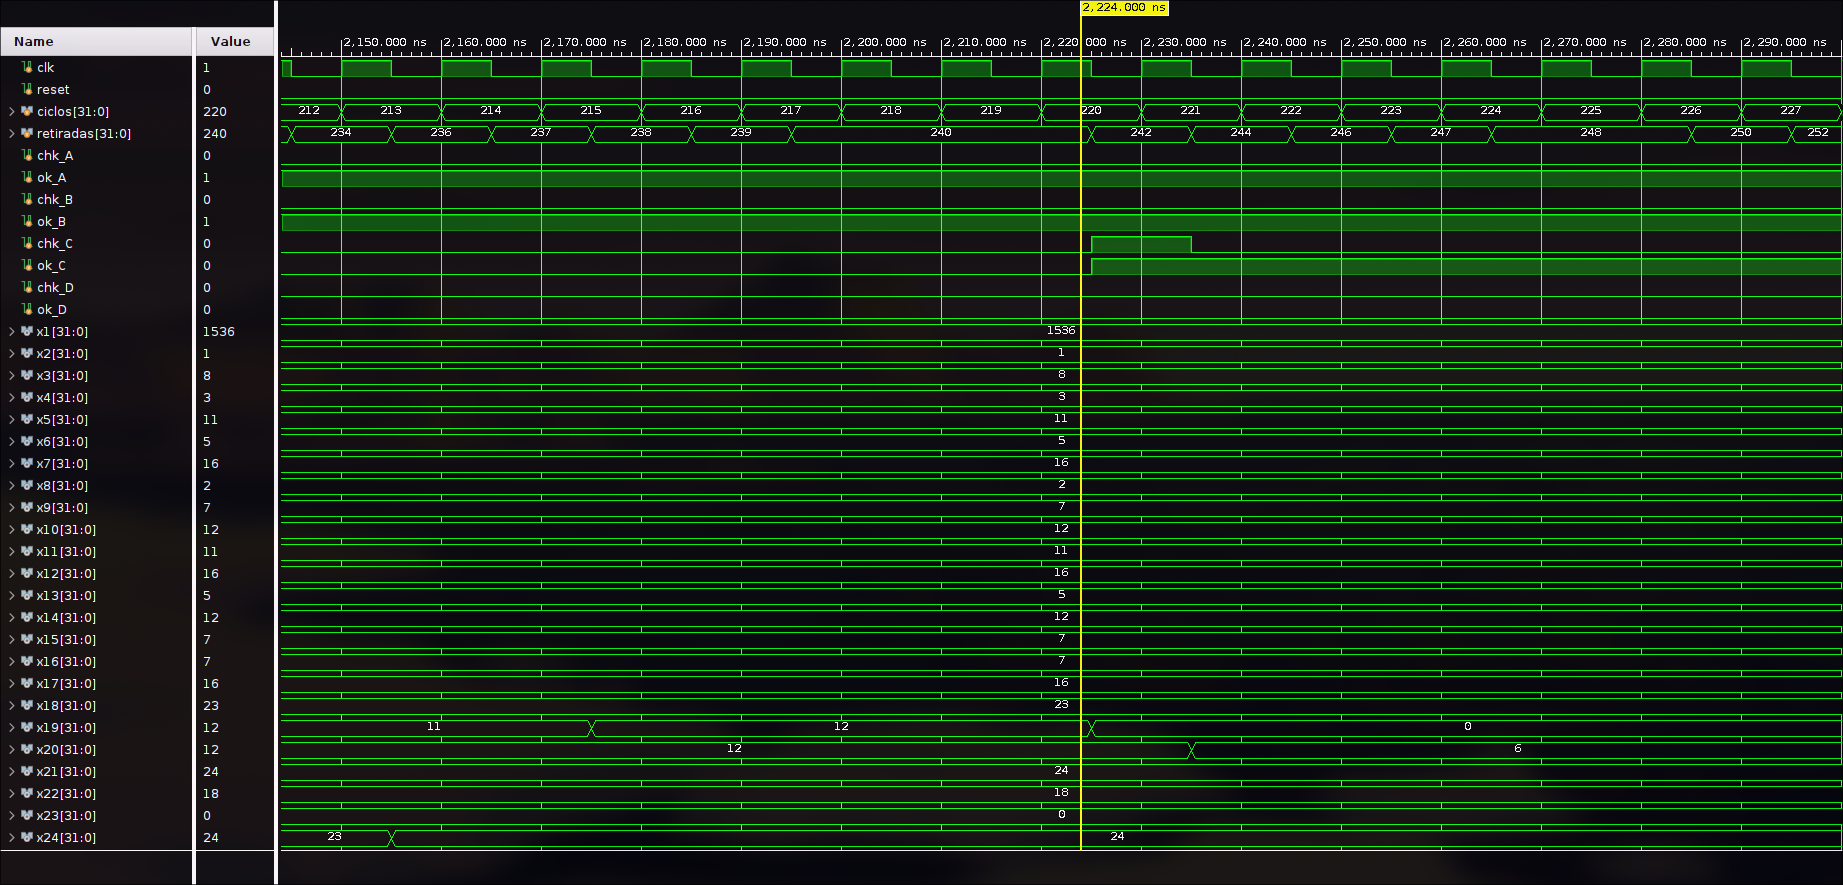
\includegraphics[width=\textwidth]{capturas/w1c_etapa_C.png}\\[2pt]
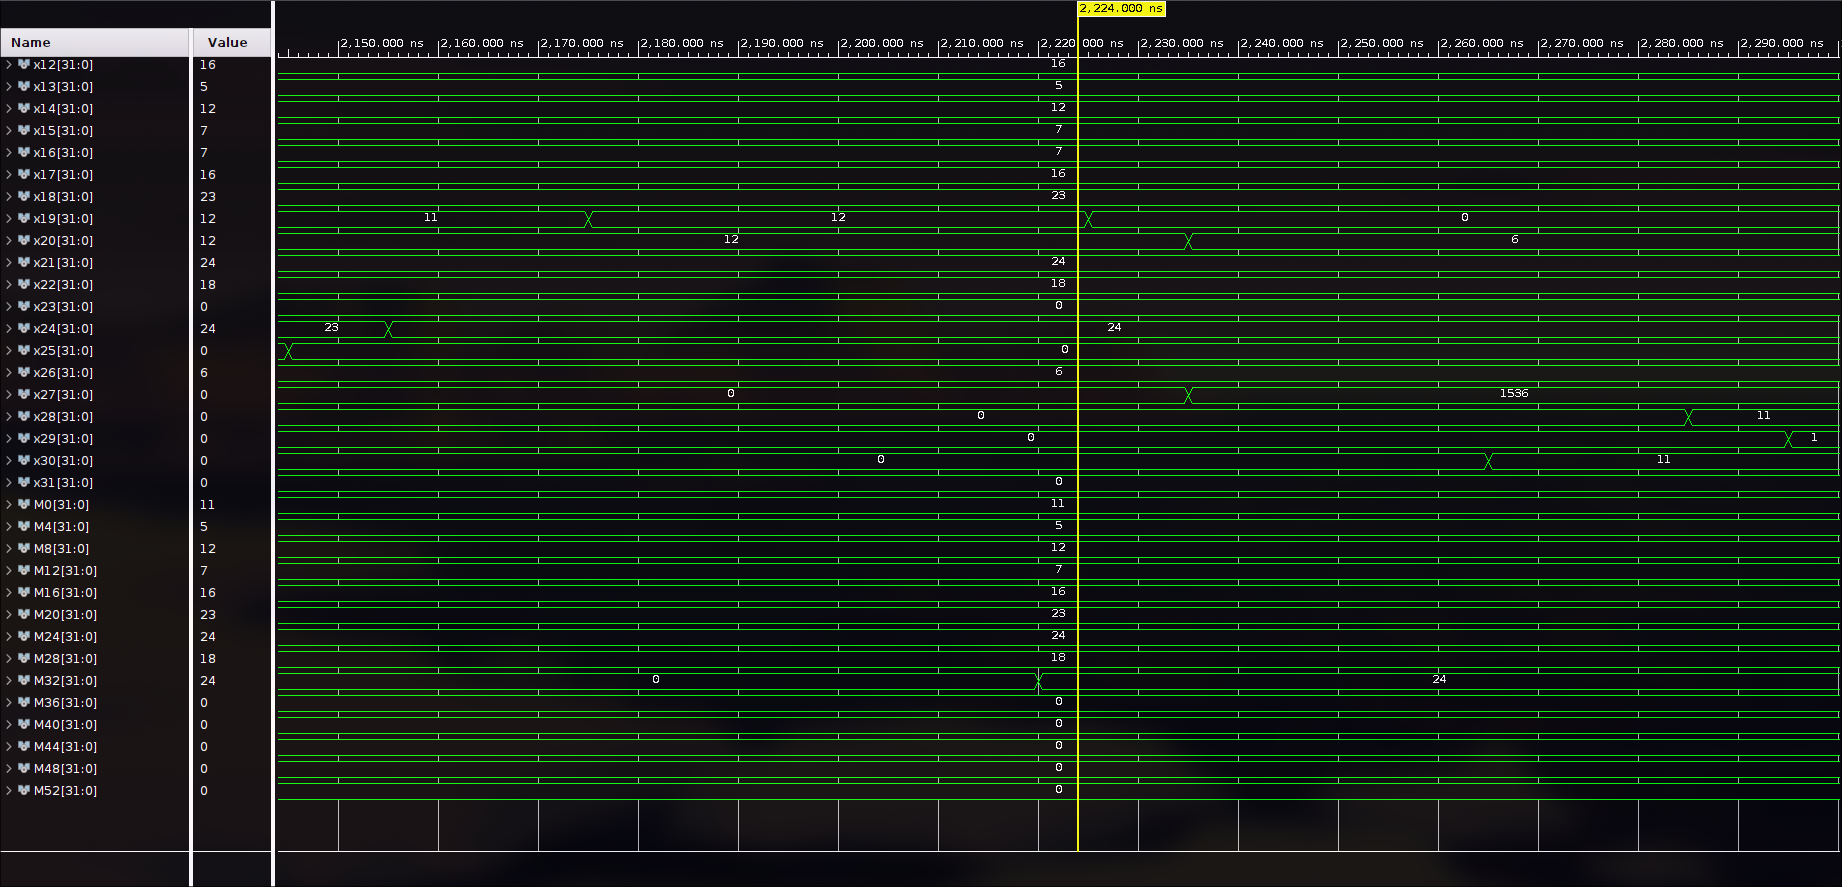
\includegraphics[width=\textwidth]{capturas/w1c_mem.png}
\caption{Cierre de la etapa C (cursor en 2224~ns, 1~ns antes del pulso \sig{chk\_C}, visible justo a la derecha del cursor). x19~=~12, x20~=~12, x21~=~24, x22~=~18, x24~=~24 y x26~=~6; M24~=~24, M28~=~18 y M32~=~24.}
\label{fig:w1c}
\end{figure}

\paragraph{Por qué el cursor de la etapa C está 1~ns antes del pulso.} En el ciclo de 2225~ns se retiran juntas, una en cada vía, la última instrucción de C (\sig{sw x24,32(x1)}, PC~224) y la primera de D (\sig{addi x19,x0,0}, PC~228). Ambas escriben el Register File en el mismo flanco de bajada, de modo que justo en 2225~ns el banco ya muestra x19~=~0. El testbench reporta \sig{ok\_C~=~1} porque verifica con el modelo de commit, exactamente entre las dos instrucciones. Por eso la captura se toma 1~ns antes del flanco. Es una consecuencia directa de la emisión doble: el final de una etapa del programa puede caer a la mitad de un paquete.

\begin{figure}[H]
\centering
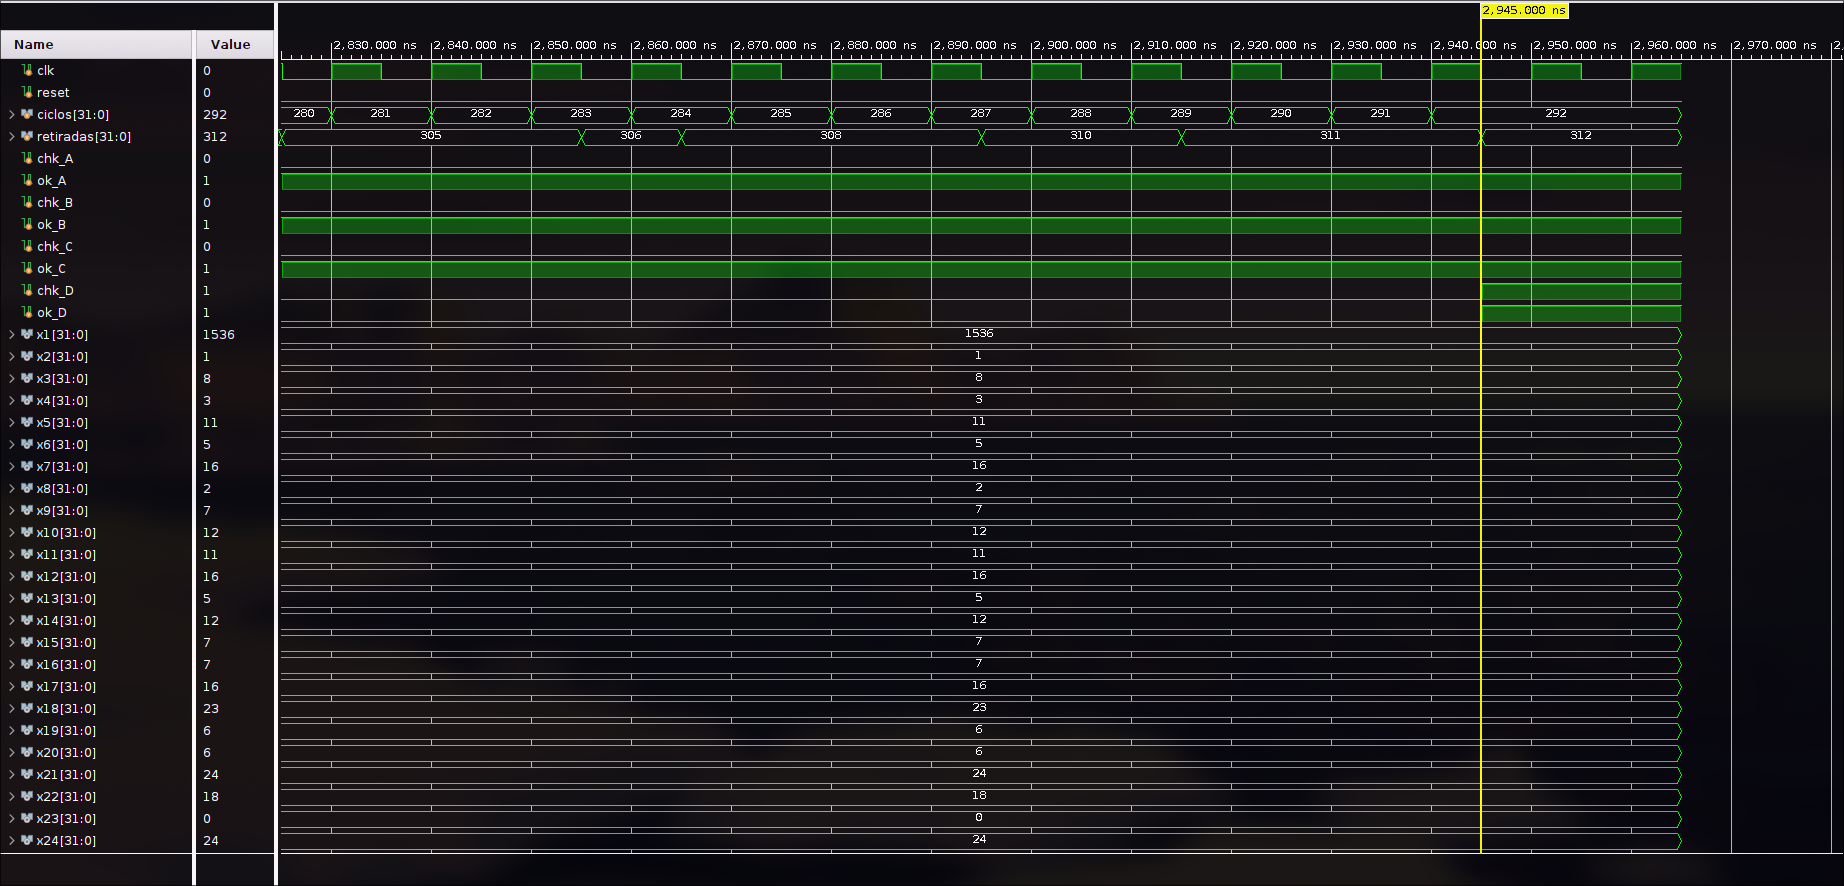
\includegraphics[width=\textwidth]{capturas/w1d_etapa_D.png}\\[2pt]
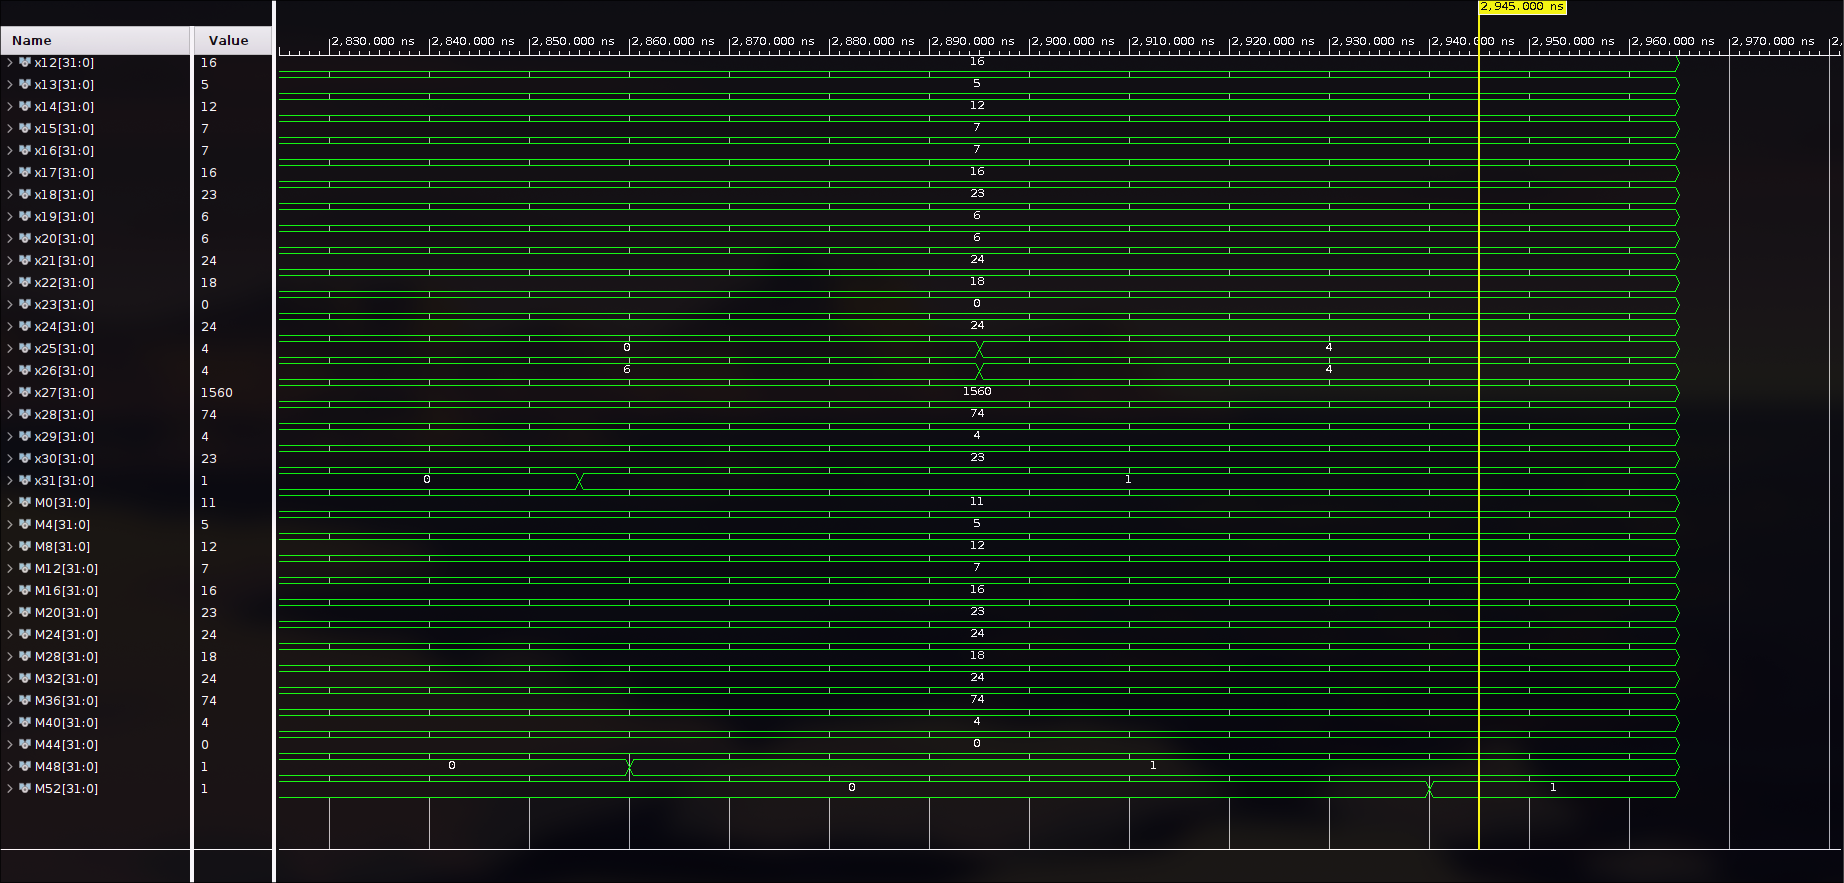
\includegraphics[width=\textwidth]{capturas/w1d_mem.png}
\caption{Cierre de la etapa D (2945~ns, ciclo 292, 312 instrucciones retiradas). x25~=~4, x26~=~4, x27~=~1560, x28~=~74, x29~=~4, x30~=~23 y x31~=~1; M36~=~74, M40~=~4, M44~=~0, M48~=~1 y M52~=~1. \sig{ok\_D~=~1}.}
\end{figure}

\subsection{Caso clave 1: doble emisión con WAW sobre x9 y prioridad de forwarding}

Instrucciones: PC~32 \sig{add x9,x7,x8}, PC~36 \sig{addi x9,x0,7}, PC~40 \sig{add x10,x9,x6}. Versión B; el comportamiento es idéntico en C.

\begin{figure}[H]
\centering
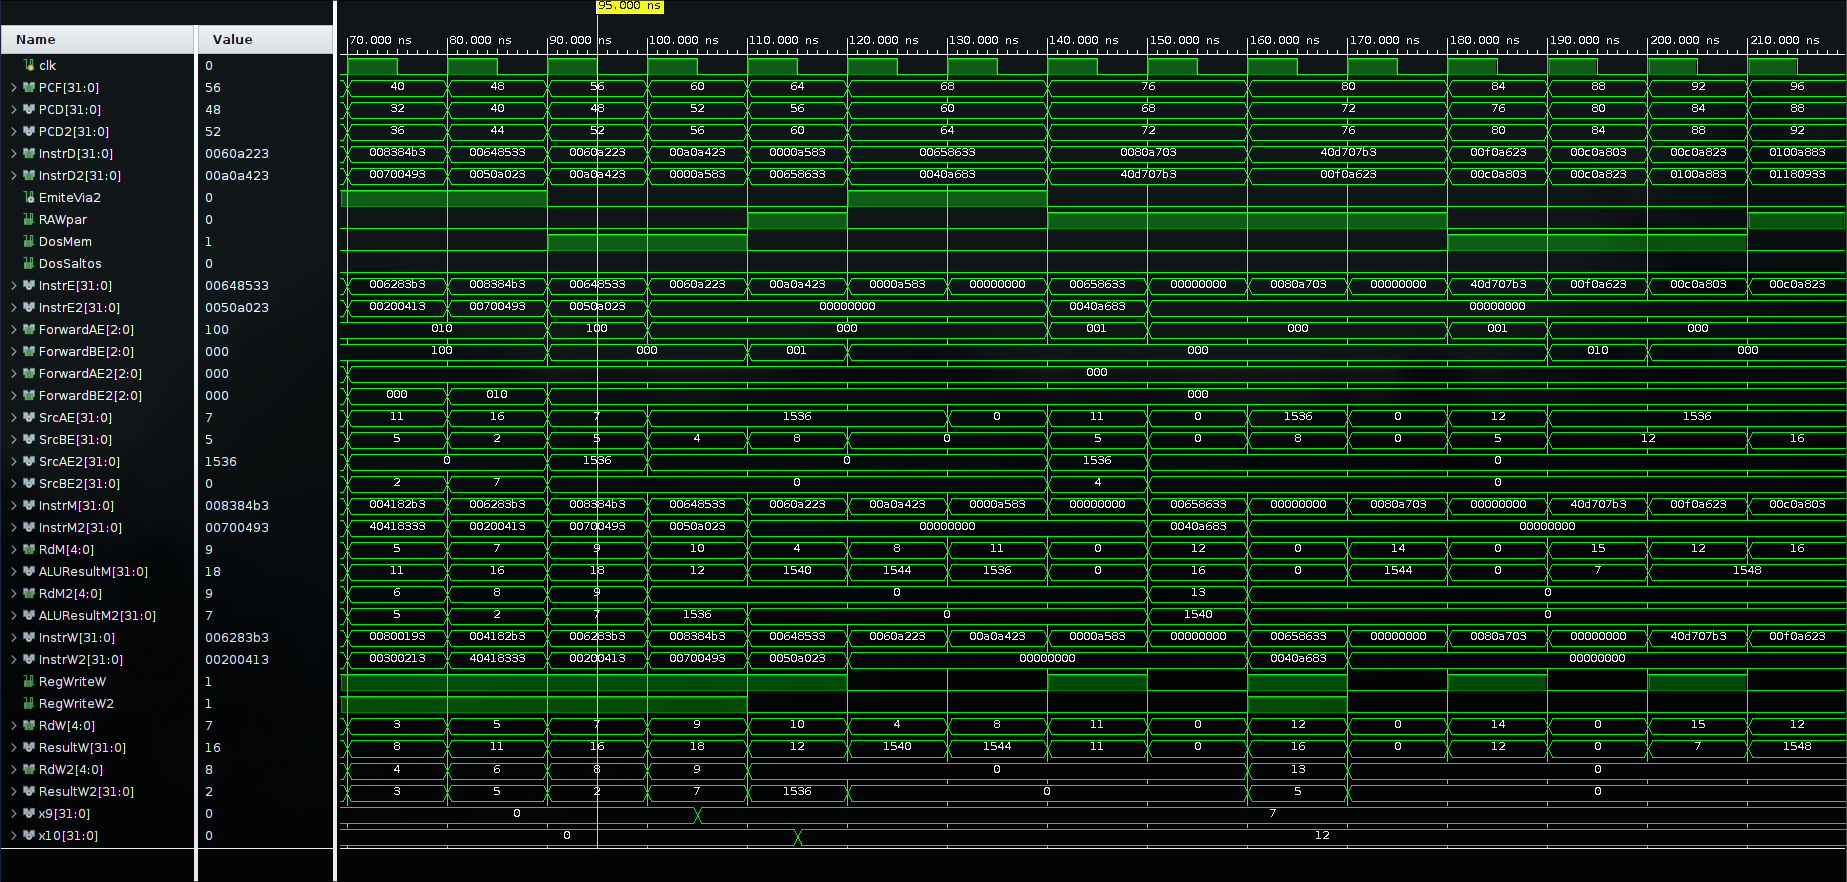
\includegraphics[width=\textwidth]{capturas/w2_zoom.png}
\caption{Doble emisión de un par con WAW y forwarding desde la vía 2 (cursor en 95~ns).}
\label{fig:w2}
\end{figure}

\begin{table}[H]
\centering
\small
\begin{tabularx}{\textwidth}{l X}
\toprule
Ciclo & Observación \\
\midrule
70–80~ns & En Decode, \sig{PCD~=~32} y \sig{PCD2~=~36}. \sig{RAWpar~=~0} porque \sig{addi x9,x0,7} no lee x9, y \sig{EmiteVia2~=~1}: el par sale junto aunque las dos instrucciones escriben el mismo registro. \\
80–90~ns & En Execute, ALU1 calcula 16~+~2~=~18 y ALU2 calcula 7. En Decode, \sig{add x10} y \sig{sw x5} también salen juntas. \\
90–100~ns & \sig{add x10} está en Execute y necesita x9. En Memory hay dos productores de x9: \sig{ALUResultM~=~18} y \sig{ALUResultM2~=~7}. \textbf{\sig{ForwardAE~=~100}} selecciona la vía 2, que es la más joven, y \sig{SrcAE~=~7}. En Decode, \sig{DosMem~=~1}: dos \sig{sw} seguidos, sale solo uno. \\
100–110~ns & En Writeback, \sig{RdW~=~9} con \sig{ResultW~=~18} y \sig{RdW2~=~9} con \sig{ResultW2~=~7}. El Register File escribe primero la vía 1 y luego la vía 2, así que \textbf{x9 queda en 7} (Figura~\ref{fig:w2b}). \\
110–120~ns & x10~=~12. Si la prioridad estuviera invertida, x10 valdría 18~+~5~=~23. Además \sig{RAWpar~=~1}: \sig{lw x11} y \sig{add x12,x11} no pueden emitirse juntas. \\
\bottomrule
\end{tabularx}
\caption{Lectura ciclo a ciclo de la Figura~\ref{fig:w2}.}
\end{table}

\begin{figure}[H]
\centering
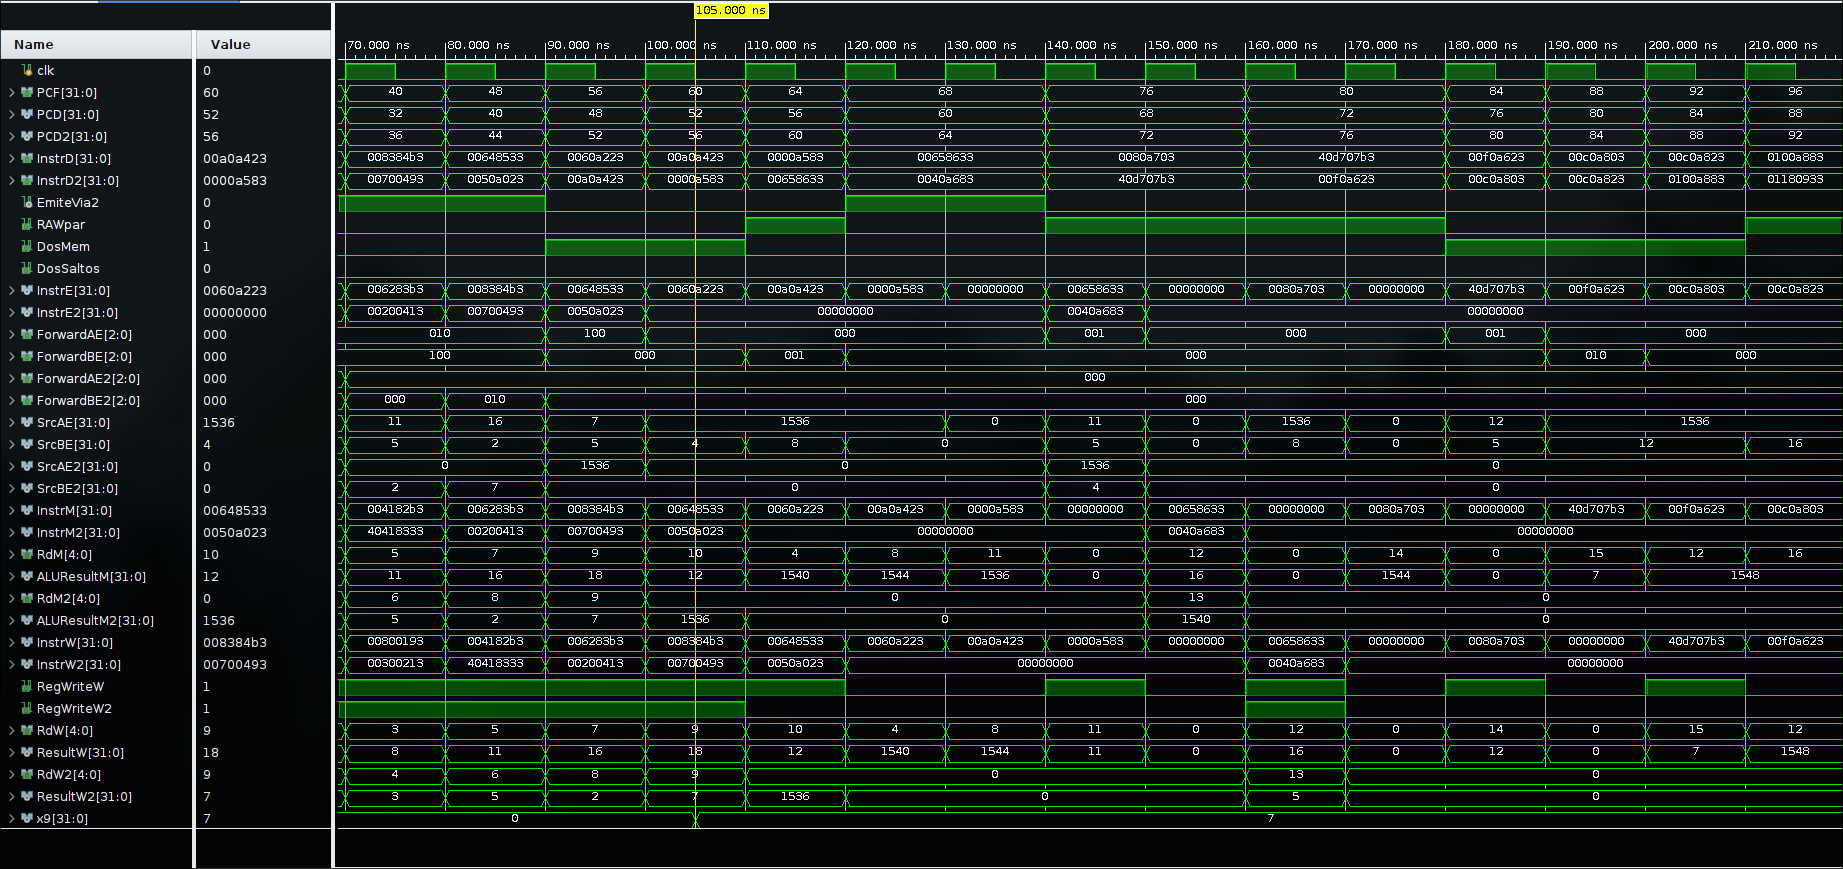
\includegraphics[width=\textwidth]{capturas/w2b_zoom.png}
\caption{Cursor en 105~ns: dos escrituras al mismo registro en el mismo ciclo; queda el valor de la vía 2.}
\label{fig:w2b}
\end{figure}

La Issue Unit solo bloquea la emisión doble ante RAW dentro del par; un WAW no la impide. La semántica secuencial se conserva en dos puntos: la prioridad del forwarding (M2~$>$~M1~$>$~W2~$>$~W1) y el orden de escritura en el Register File.

\subsection{Caso clave 2: load-use en el lazo D1}

Instrucciones: PC~252 \sig{lw x30,0(x27)}, PC~256 \sig{add x28,x28,x30}, PC~260 \sig{slt x25,x30,x5}. Primera iteración de D1, versión B.

\begin{figure}[H]
\centering
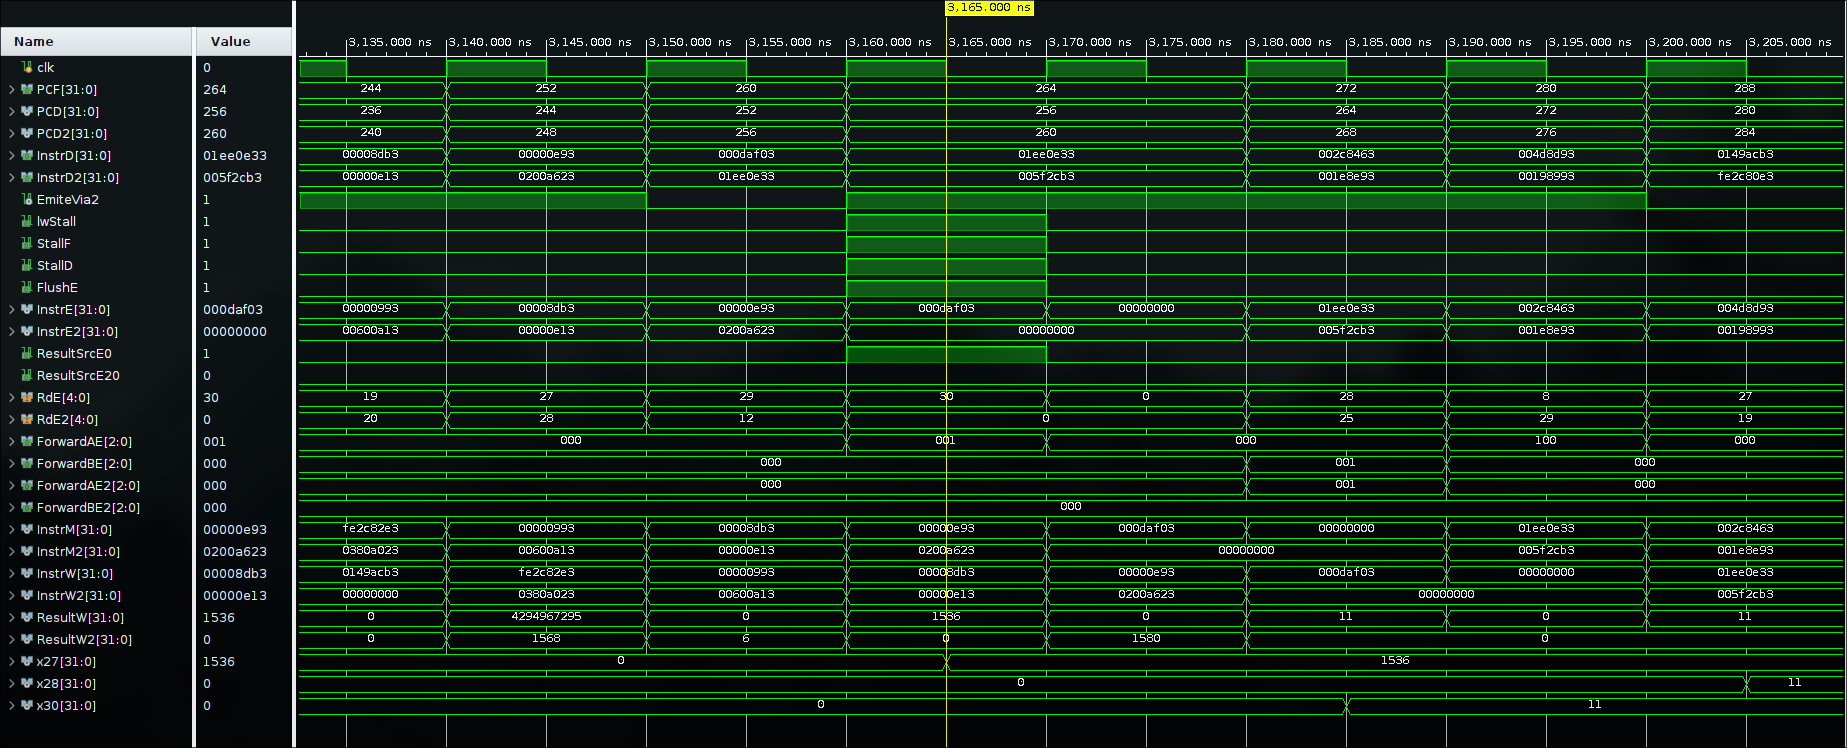
\includegraphics[width=\textwidth]{capturas/w3_zoom.png}
\caption{Emisión parcial por RAW, stall por load-use y forwarding de un mismo productor a las dos vías (cursor en 3165~ns).}
\label{fig:w3}
\end{figure}

\begin{table}[H]
\centering
\small
\begin{tabularx}{\textwidth}{l X}
\toprule
Ciclo & Observación \\
\midrule
3150–3160~ns & En Decode, \sig{PCD~=~252} (\sig{lw}) y \sig{PCD2~=~256} (\sig{add}). Hay RAW dentro del par, así que \sig{EmiteVia2~=~0} y sale solo el \sig{lw}. El \sig{add} se reagrupa como vía 1 y entra 260 (\sig{slt}) como vía 2. \\
3160–3170~ns & El \sig{lw} está en Execute (\sig{ResultSrcE0~=~1}, \sig{RdE~=~30}) y las dos instrucciones de Decode usan x30: \textbf{\sig{lwStall~=~StallF~=~StallD~=~FlushE~=~1}}. El PC se congela en 264. \\
3170–3180~ns & Burbuja: \sig{InstrE~=~InstrE2~=~0}. El \sig{lw} está en Memory leyendo la memoria. \\
3180–3190~ns & \sig{add} y \sig{slt} salen juntas. El \sig{lw} está en Writeback con x30~=~11: \sig{ForwardBE~=~001} (para el \sig{add}) y \sig{ForwardAE2~=~001} (para el \sig{slt}) toman \sig{ResultW}. \\
\bottomrule
\end{tabularx}
\caption{Lectura ciclo a ciclo de la Figura~\ref{fig:w3}.}
\end{table}

En el Dual-Issue un load-use cuesta doble: primero la Issue Unit separa el par por RAW y luego la Hazard Unit inserta una burbuja. Cada iteración de D1 pierde unos tres slots de emisión.

\subsection{Prueba específica de la optimización (\texttt{prog6\_prediccion})}

El programa es un lazo de 10 iteraciones que contiene dos saltos con comportamientos opuestos: PC~48 (\sig{beq x7,x5,L}) es el salto del lazo, tomado 9 veces y no tomado 1 vez; PC~32 (\sig{beq x4,x5,S}) alterna tomado y no tomado en cada iteración.

\begin{figure}[H]
\centering
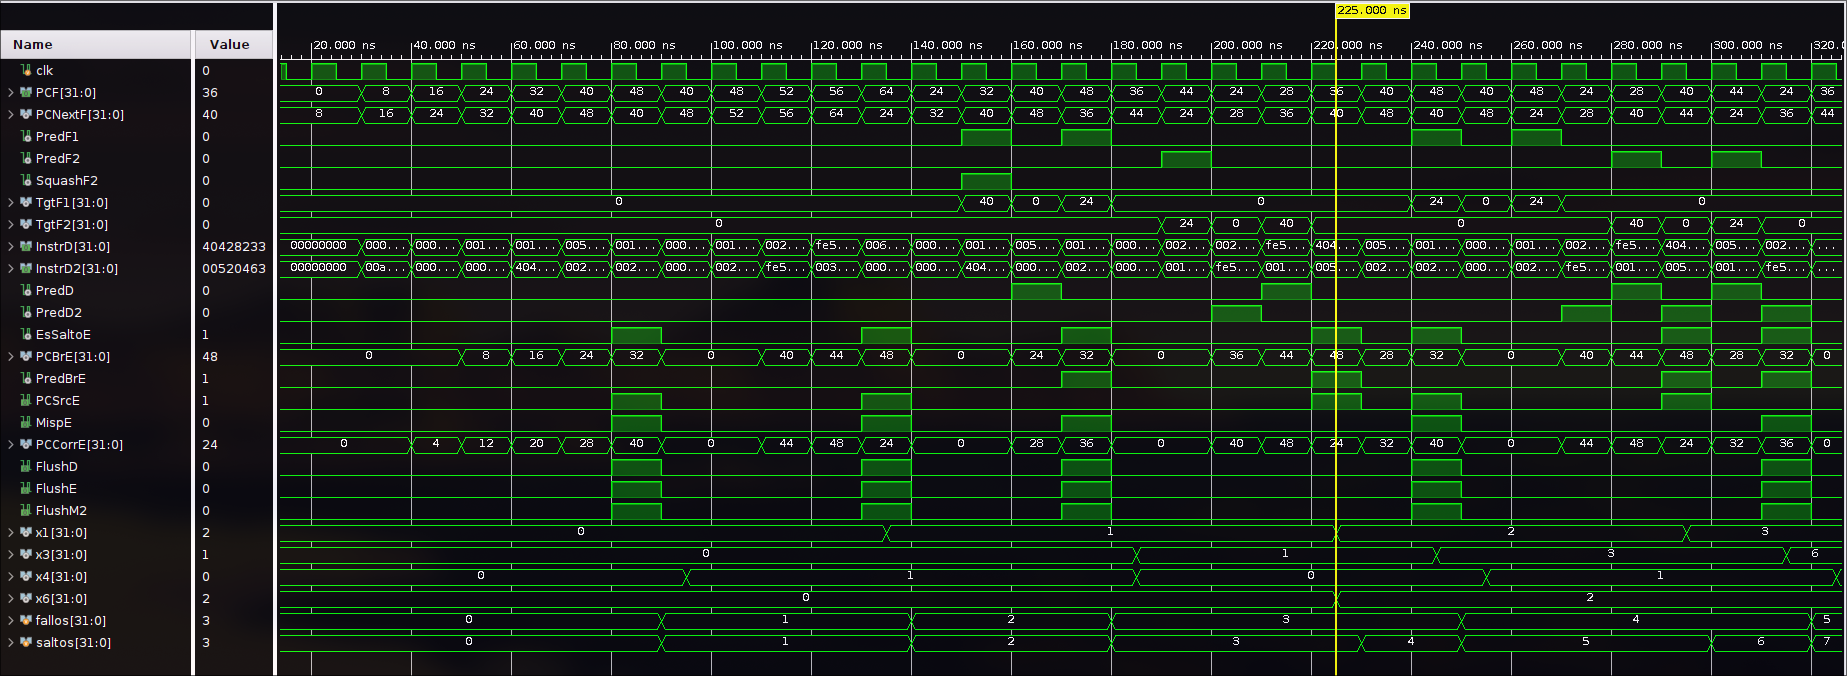
\includegraphics[width=\textwidth]{capturas/w4_zoom.png}
\caption{Funcionamiento del BTB (versión C). Cursor en 225~ns: acierto en el salto del lazo.}
\label{fig:w4}
\end{figure}

\begin{table}[H]
\centering
\small
\begin{tabularx}{\textwidth}{cccccc X}
\toprule
Tiempo & PC salto & \sig{PredBrE} & \sig{PCSrcE} & \sig{MispE} & \sig{PCCorrE} & Interpretación \\
\midrule
85~ns & 32 & 0 & 1 & 1 & 40 & Fallo en frío: el BTB está vacío; se crea la entrada \\
135~ns & 48 & 0 & 1 & 1 & 24 & Fallo en frío del salto del lazo \\
175~ns & 32 & 1 & 0 & 1 & 36 & Predijo tomado y no salta: corrección a PC+4 \\
\textbf{225~ns} & \textbf{48} & \textbf{1} & \textbf{1} & \textbf{0} & — & \textbf{Acierto: no hay flush} \\
245~ns & 32 & 0 & 1 & 1 & 40 & El contador bajó a 01 y el salto vuelve a tomarse \\
275~ns & 48 & 1 & 1 & 0 & — & Acierto \\
\bottomrule
\end{tabularx}
\caption{Saltos resueltos en Execute en la Figura~\ref{fig:w4}.}
\end{table}

En Fetch ya se ve la predicción antes de que el salto llegue a Execute. Entre 140 y 150~ns aparecen \sig{PredF1~=~1}, \sig{TgtF1~=~40} y \sig{SquashF2~=~1}, y el PC salta directamente al destino. En los aciertos (225 y 275~ns), \sig{FlushD} y \sig{FlushE} quedan en 0. Al final, el salto del lazo falla 2 de 10 veces (arranque en frío y salida) y el alternante falla 10 de 10: el contador oscila entre 01 y 10 y siempre predice lo contrario de lo que pasa.

\section{Programa propio}

\subsection{Descripción}

El programa trabaja sobre un arreglo \sig{A[16]} en la dirección 1024, \sig{B} en 1088, \sig{C} en 1152 y los resultados en 1216. Ejecuta 490 instrucciones (101 estáticas) en cuatro etapas, cada una con su checkpoint:

\begin{enumerate}[nosep]
  \item \textbf{Inicialización con software pipelining}: se intercala el \sig{addi} de la siguiente constante con el \sig{sw} de la anterior, así cada par ALU~+~store se emite junto.
  \item \textbf{Recorrido con salto dependiente de datos}: \sig{B[i]~=~A[i]~+~i}, suma total y conteo de \sig{A[i]~>~7}. El patrón del salto (N N T T N T N T N T N T T N T N) es irregular: es el caso difícil para el predictor.
  \item \textbf{Suma vectorial desenrollada $\times$2}: \sig{C~=~A~+~B} con dos cadenas independientes por iteración, lo que da más ILP y un salto de lazo predecible.
  \item \textbf{Lazos anidados 4$\times$4}: suma por filas de \sig{C} y máximo. El salto interno falla una vez por cada salida.
\end{enumerate}

Estado final verificado: suma~=~120, conteo~=~8, filas de \sig{C}~=~68, 82, 104 y 106, y máximo~=~106. Las tres versiones pasan los cuatro checkpoints.

\section{Comparación cuantitativa}

\begin{table}[H]
\centering
\small
\begin{tabular}{lrrr@{\hspace{18pt}}rrr}
\toprule
 & \multicolumn{3}{c}{Programa del profesor} & \multicolumn{3}{c}{Programa propio} \\
\cmidrule(lr){2-4}\cmidrule(lr){5-7}
Indicador & A & B & C & A & B & C \\
\midrule
Ciclos totales & 458 & 387 & 292 & 583 & 437 & 373 \\
Instrucciones retiradas & 312 & 312 & 312 & 490 & 490 & 490 \\
CPI & 1.468 & 1.240 & 0.936 & 1.190 & 0.892 & 0.761 \\
IPC & 0.681 & 0.806 & 1.068 & 0.840 & 1.121 & 1.314 \\
Speedup vs.\ A & 1.00 & 1.18 & 1.57 & 1.00 & 1.33 & 1.56 \\
Speedup vs.\ B & — & 1.00 & 1.33 & — & 1.00 & 1.17 \\
\midrule
Ciclos con stall load-use & 9 & 11 & 12 & 0 & 48 & 41 \\
Flushes por salto & 68 & 68 & 33 & 46 & 46 & 25 \\
Ciclos con dos retiros & 0 & 74 & 99 & 0 & 195 & 209 \\
Precisión del predictor & — & — & 63.3\,\% & — & — & 61.5\,\% \\
\bottomrule
\end{tabular}
\caption{Comparación de las tres arquitecturas. Los flushes y la precisión incluyen el \sig{jal x0,fin}, que llega a Execute antes de que se retire la última instrucción útil.}
\label{tab:comparacion}
\end{table}

\begin{figure}[H]
\centering
\begin{tikzpicture}
\begin{axis}[ybar, bar width=16pt, width=0.85\textwidth, height=6.2cm, ymin=0, ymax=650,
  symbolic x coords={Profesor, Propio}, xtick=data, enlarge x limits=0.45,
  ylabel={Ciclos}, legend style={at={(0.5,1.03)}, anchor=south, legend columns=3, draw=none},
  nodes near coords, nodes near coords style={font=\footnotesize}, every axis plot/.append style={draw=none}]
\addplot[fill=gray!55] coordinates {(Profesor,458) (Propio,583)};
\addplot[fill=blue!45] coordinates {(Profesor,387) (Propio,437)};
\addplot[fill=nuevo!80] coordinates {(Profesor,292) (Propio,373)};
\legend{A — Pipeline, B — Dual-Issue, C — Optimizado}
\end{axis}
\end{tikzpicture}
\caption{Ciclos totales por arquitectura y programa.}
\end{figure}

\subsection{Fallos de predicción por salto}

\begin{table}[H]
\centering
\footnotesize
\setlength{\tabcolsep}{4pt}
\begin{tabular}{rllrrrl}
\toprule
PC & Programa & Salto & Ejec. & Tom. & Fallos & Causa \\
\midrule
124 & Profesor & \sig{beq x25,x2,C1} & 12 & 11 & 2 & frío y salida del lazo \\
148 & Profesor & \sig{beq x23,x2,C2a} & 12 & 6 & \textbf{12} & patrón alternante T/NT \\
172 & Profesor & \sig{beq x25,x2,C2} & 12 & 11 & 2 & frío y salida \\
196 & Profesor & \sig{beq x25,x2,C3a} & 12 & 6 & 3 & 6 T y luego 6 NT: transición \\
220 & Profesor & \sig{beq x25,x2,C3} & 12 & 11 & 2 & frío y salida \\
264 & Profesor & \sig{beq x25,x2,D2} & 6 & 2 & 4 & depende de los datos \\
284 & Profesor & \sig{beq x25,x2,D1} & 6 & 5 & 2 & frío y salida \\
— & Profesor & \sig{jal}, D3–D6 y \sig{fin} & 18 & — & 6 & frío o ejecución única \\
\midrule
208 & Propio & \sig{beq x22,x0,L2s} & 16 & 8 & \textbf{13} & \sig{A[i]~>~7}, irregular \\
220 & Propio & \sig{beq x23,x15,L2} & 16 & 15 & 2 & frío y salida \\
304 & Propio & \sig{beq x23,x15,L3} & 8 & 7 & 2 & frío y salida \\
356 & Propio & \sig{beq x23,x15,L4i} & 16 & 12 & 5 & salida en cada iteración externa \\
368 & Propio & \sig{beq x29,x0,L4n} & 4 & 0 & 0 & nunca se toma: no entra al BTB \\
388 & Propio & \sig{beq x23,x15,L4o} & 4 & 3 & 2 & frío y salida \\
400 & Propio & \sig{jal x0,fin} & 1 & 1 & 1 & frío \\
\bottomrule
\end{tabular}
\caption{Comportamiento del predictor por salto en la versión C.}
\label{tab:saltos}
\end{table}

\section{Análisis}

\subsection{Mejora del Dual-Issue frente al pipeline}

B mejora a A en 1.18$\times$ (profesor) y 1.33$\times$ (propio). La diferencia entre los dos programas se explica por cuánto paralelismo independiente tiene cada uno. El programa propio tiene más pares ALU~+~memoria e instrucciones independientes (195 ciclos con dos retiros), mientras que el del profesor está dominado por cadenas \sig{addi}~$\rightarrow$~\sig{slt}~$\rightarrow$~\sig{beq} que no pueden emparejarse.

Un efecto menos evidente es que el load-use cuesta más con emisión doble. En el programa propio, A no tiene ningún stall load-use porque el consumidor de cada \sig{lw} está dos instrucciones después. En B aparecen 48: esas dos instrucciones se emiten en ciclos consecutivos, así que el \sig{lw} y su consumidor quedan en paquetes contiguos. La distancia que basta en un pipeline escalar no basta con emisión doble.

\subsection{Por qué no se alcanza el IPC ideal de 2}

Para separar lo que corresponde al predictor de lo que es estructural, se calculó con un modelo de la traza dinámica el número de ciclos que tendría un procesador con las mismas reglas de emisión que nuestra Issue Unit y un \textbf{predictor perfecto}:

\begin{table}[H]
\centering
\begin{tabular}{lcccc}
\toprule
 & B & C & Predictor perfecto & IPC ideal \\
\midrule
Programa del profesor (CPI) & 1.240 & 0.936 & $\approx$\,0.81 & 0.50 \\
Programa propio (CPI) & 0.892 & 0.761 & $\approx$\,0.66 & 0.50 \\
\bottomrule
\end{tabular}
\caption{CPI medido y cotas. La columna «Predictor perfecto» es una estimación del modelo, no una simulación del RTL.}
\end{table}

Aun con predicción perfecta, el CPI no baja de $\approx$\,0.81 en el programa del profesor, por cuatro motivos:
\begin{enumerate}[nosep]
  \item Dependencias RAW dentro del par: cada lazo tiene la cadena \sig{addi x19}~$\rightarrow$~\sig{slt x25}~$\rightarrow$~\sig{beq x25}, y cada eslabón obliga a emitir solo una instrucción.
  \item Un único puerto de memoria: la etapa B es casi toda \sig{lw}/\sig{sw} consecutivos.
  \item Load-use: en cada iteración de D1, el \sig{lw x30} cuesta una separación del par y una burbuja.
  \item Un salto tomado en el slot 1 cierra el paquete, porque lo que viene detrás es camino incorrecto.
\end{enumerate}

\subsection{Impacto de la optimización}

El BTB reduce los flushes por salto de 68 a 33 (profesor) y de 46 a 25 (propio), lo que da un speedup de 1.33$\times$ y 1.17$\times$ respecto de B. Medido contra la cota de predictor perfecto, C recorre el 71\,\% de la distancia entre B y esa cota en el programa del profesor y el 57\,\% en el propio. El resto son fallos del predictor.

La mejora es mayor en el programa del profesor porque tiene más saltos tomados por instrucción (67 de 312, frente a 45 de 490) y porque la mayoría están en lazos regulares (C1, C2, C3, D1), que el contador de 2 bits aprende tras una iteración. Los ciclos con doble retiro también suben (74~$\rightarrow$~99 y 195~$\rightarrow$~209): al no vaciarse el pipeline, la Issue Unit recibe más pares válidos.

\subsection{Cuándo la optimización es útil y cuándo no}

\begin{itemize}[nosep]
  \item \textbf{Útil:} lazos con muchas iteraciones y saltos con sesgo estable. Los saltos de lazo fallan solo dos veces (frío y salida) y los \sig{jal} solo la primera vez.
  \item \textbf{No útil:}
    \begin{itemize}[nosep]
      \item Patrones alternantes. \sig{beq x23,x2,C2a} y el salto de \sig{prog6} fallan el 100\,\% de las veces: el contador de 2 bits no tiene historia, solo sesgo.
      \item Saltos que dependen de datos sin patrón: \sig{A[i]~>~7} falla 13 de 16 veces.
      \item Código que se ejecuta una sola vez: los saltos de D3–D6 son fallos en frío obligatorios.
    \end{itemize}
  \item \textbf{Puede empeorar en saltos concretos:} en B un salto no tomado no cuesta nada, mientras que en C cuesta un flush si se había predicho tomado. El \sig{beq} alternante de C2 provoca 12 flushes en C frente a 6 en B. En el balance global gana C porque los saltos de lazo dominan. Un salto que nunca se toma no entra al BTB, así que no genera predicciones erróneas.
  \item \textbf{Costo:} 976 bits de almacenamiento más 132 flip-flops y la lógica de comparación, además de más retardo en Fetch.
\end{itemize}

\section{Conclusiones y trabajo futuro}

\begin{itemize}
  \item Las tres arquitecturas son funcionalmente equivalentes. Así lo demuestran los checkpoints de los dos programas, los testbenches de E2, 400 programas aleatorios contra un modelo ISA y la reproducción en Vivado.
  \item El Dual-Issue mejora al pipeline entre 1.18$\times$ y 1.33$\times$. El IPC queda lejos de 2 por las dependencias, el puerto único de memoria, los load-use y, sobre todo, los saltos.
  \item El BTB con predictor de 2 bits elimina aproximadamente la mitad de los flushes y lleva el speedup total frente al pipeline a 1.57$\times$ y 1.56$\times$, con un IPC superior a 1 en los dos programas.
  \item La principal limitación es la falta de historia: los patrones alternantes y los saltos que dependen de datos siguen fallando.
\end{itemize}

\textbf{Trabajo futuro:}
\begin{enumerate}[nosep]
  \item Un predictor con historia global (por ejemplo, gshare) para capturar patrones alternantes como el de C2.
  \item Resolver los saltos en Decode para reducir a un ciclo el costo de cada fallo.
  \item Una Instruction Queue que desacople Fetch de la emisión y aproveche los ciclos con una sola instrucción emitida.
  \item Reordenamiento estático (por el compilador) para separar los \sig{lw} de sus consumidores al menos dos paquetes.
\end{enumerate}

\appendix
\sloppy
\section{Reproducción}

Repositorio: \url{https://github.com/pepitoAE/Duall-Proccesor}. Cada versión está en su carpeta (\sig{A\_single\_issue}, \sig{B\_dual\_issue}, \sig{C\_dual\_optimizado}), con \sig{src/}, \sig{sim/} y \sig{mem/}.

\begin{itemize}[nosep]
  \item \sig{bash vivado/correr\_xsim.sh} compila y simula los testbenches de los dos programas en las tres versiones y \sig{prog6} en B y C, y deja el resumen en \sig{vivado/xsim\_runs/resumen.txt}.
  \item \sig{bash vivado/ondas.sh N} (N = 1…4) abre las waveforms de este informe con las señales ya configuradas.
  \item \sig{tools/asm.py} es el ensamblador, \sig{tools/modelo\_isa.py} el modelo de referencia, \sig{tools/gen\_tb.py} genera testbenches con checkpoints y \sig{tools/fuzz/} contiene la prueba diferencial aleatoria.
\end{itemize}

\end{document}
